% Created 2025-01-16 do 13:24
% Intended LaTeX compiler: pdflatex
\documentclass[11pt]{article}
\usepackage[utf8]{inputenc}
\usepackage[T1]{fontenc}
\usepackage{graphicx}
\usepackage{longtable}
\usepackage{wrapfig}
\usepackage{rotating}
\usepackage[normalem]{ulem}
\usepackage{amsmath}
\usepackage{amssymb}
\usepackage{capt-of}
\usepackage{hyperref}
\author{Music Player Daemon (MPD) user}
\date{\today}
\title{SSS/GNU system - Manual \& Documentation}
\hypersetup{
 pdfauthor={Music Player Daemon (MPD) user},
 pdftitle={SSS/GNU system - Manual \& Documentation},
 pdfkeywords={},
 pdfsubject={},
 pdfcreator={Emacs 29.4 (Org mode 9.6.15)}, 
 pdflang={English}}
\begin{document}

\maketitle
\tableofcontents

You are reading the manual for the Supreme Sexp System (SSS).

This manual documents the SSS/GNU system and its functionalities.

SSS is a Lisp machine adventure, where the hacking culture is celebrated. Let me help you achieve \emph{GNUrvana}.

If you like my work, please support me by \href{https://bmc.link/jjbigorra}{buying me a cup of coffee} so I can continue with a lot of motivation.

This custom GNU + Linux setup enhances customization to infinity, encourages the hacking spirit, and offers a superior user experience thanks in part too to REPL (Read Eval Print Loop) and Lisps.

Installing and managing SSS is not intended for beginners to GNU/Linux systems, and requires some prior experience in this. Familiarity with Lisp dialects is also a great plus point.

SSS strives to have all things configured via Lisp dialects when possible and convenient, staying accessible to all kinds of users, and allowing for magical things to happen.

\begin{center}
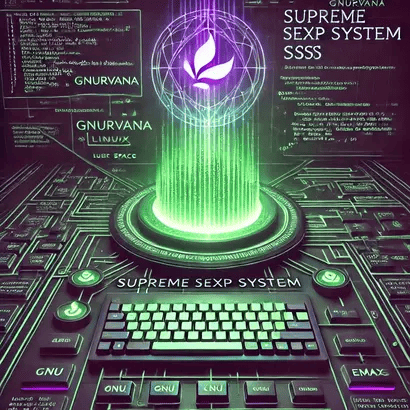
\includegraphics[width=.9\linewidth]{../../resources/images/dall-e-3-thumb.png}
\end{center}

I would appreciate if you write your findings when using SSS and if you can, fork the project, and contribute some improvements, or mail me at <jjbigorra@gmail.com>

Note: Screenshot below might be outdated and no longer representative of the current, ever-changing state of SSS.

\begin{center}
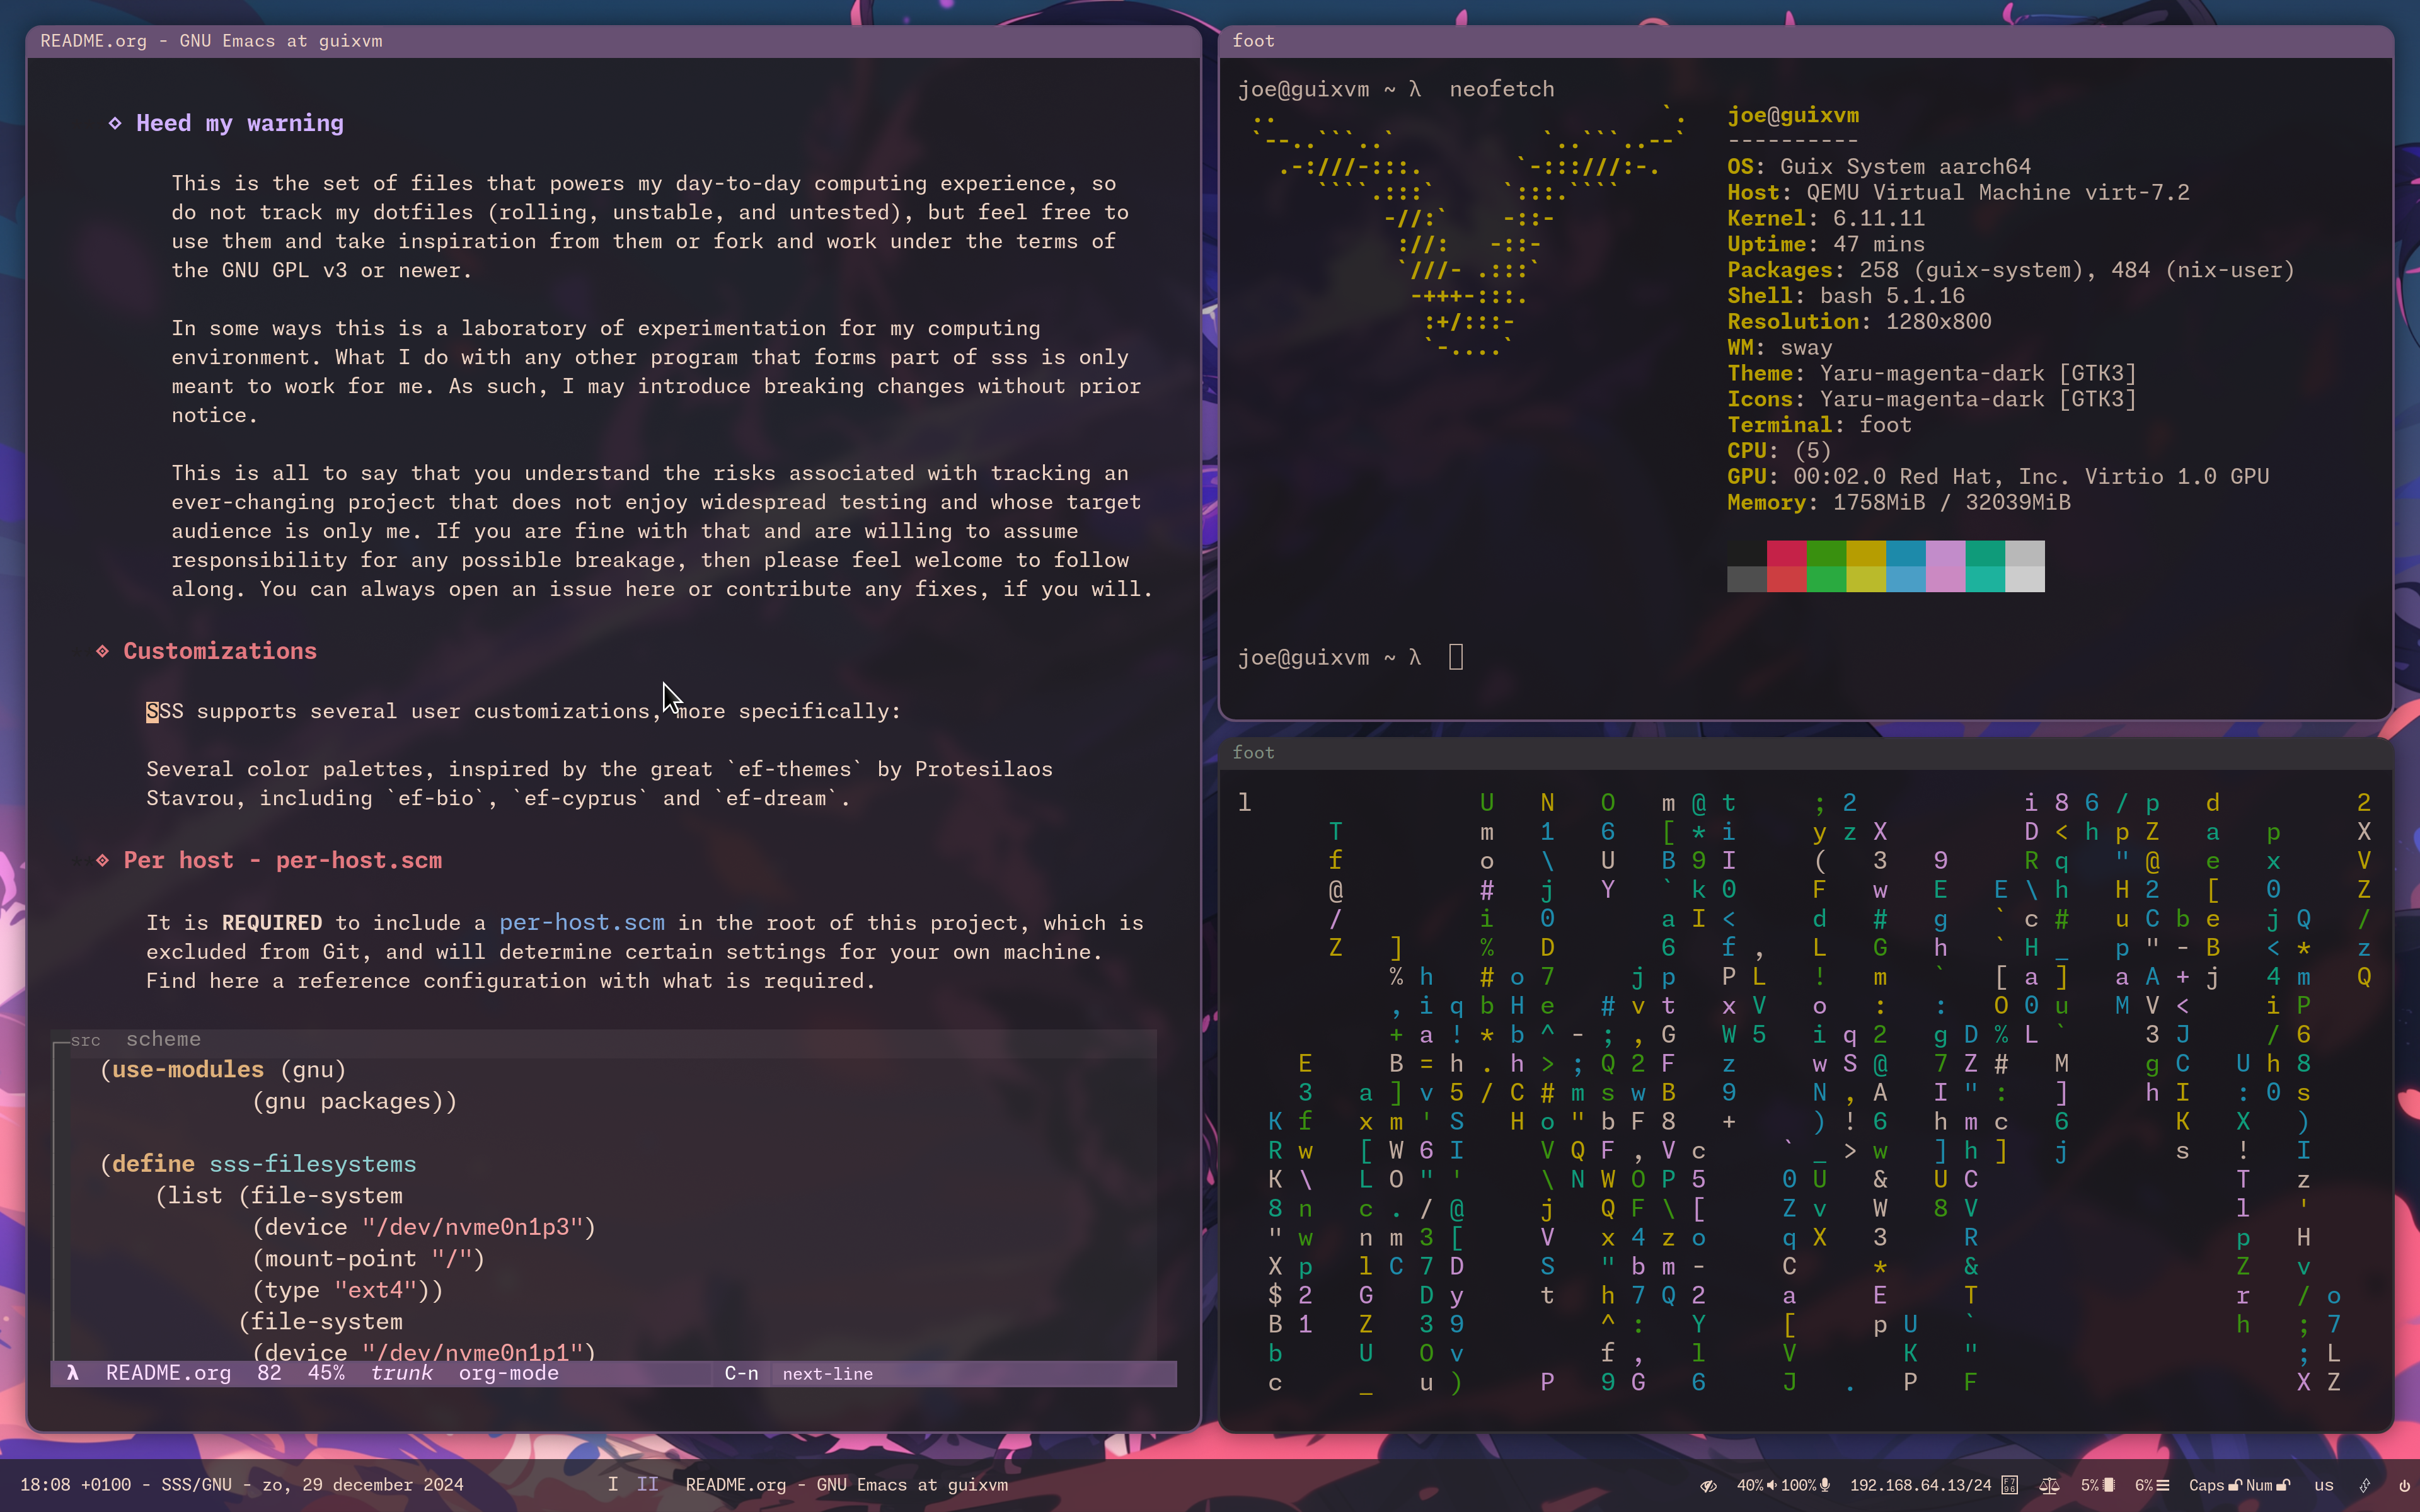
\includegraphics[width=.9\linewidth]{../../resources/screenshots/2024-12-29T18:08:55,108562468+01:00.png}
\end{center}

\section{What lies here?}
\label{sec:org78fea6c}

\subsection{An operating system (OS) configured in Scheme}
\label{sec:org086b15e}

\begin{itemize}
\item GNU Guix system configurations
\item SwayFX configurations
\item Foot terminal emulator
\item Rofi application launcher
\item Waybar configuration and style
\item Mako configuration and style
\item multi-user Git configuration setup (work/personal)
\item Qutebrowser configurations
\item Multi user configurations
\item Theme palettes that affect the entire system
\end{itemize}

\subsection{Joe's Emacs configuration}
\label{sec:org6a78d1f}

An operating system unto itself.

\begin{itemize}
\item Advanced Emacs configurations with Emacs Lisp + Elpaca
\end{itemize}

\section{Why ?}
\label{sec:orgf5e2e11}

Find the divine sayings, and the destined computer configurations, all my Guix, Scheme, SwayFX, and Emacs Lisp and more configurations here for learning you a fully Lisp machine with GNU/Linux for a great good.

Warning: parts of the code and settings might default to the Dutch language ( \texttt{nl\_NL.UTF-8} ).


I am currently working on the GNU operating system in order to create a secure libre Lisp workstation.

I refer to SSS lovingly as the modern Lisp machine. With this one obtains a computing style and programming environment that can be referred to as Lisp user space. This is a modern iteration of the Lisp machines of yore.

Staying as libre as possible, any of the system's application code can be made available to you at any time.

You can be aware of all the code that is running on your machine, which puts GNU among the most secure operating systems on Earth.

Learning Lisps is really going down a rabbit hole, but trust me, you will come out with a better understanding of programming as a whole out the other end.

Secure yourself against malevolent state actors and never trust someone else's unverified binaries again, as you can build from the source all the way down.

Lisp user space provides an introspective, hackable, and transactionable operating system that can be modified live in a REPL.

The lines between data and code fade, allowing insane flexibility and power.

Lisp user space is centered on text-based user interfaces instead of graphical user interfaces, and can be mostly used without a mouse, which makes it easier to use for people living with disabilities as well as power users.

All of the system can be inspected and most of it can be hacked live in a REPL, making it a pure expression of the libre software ethic, and an incredibly versatile tool for a skilled programmer.

In some ways this is a laboratory of experimentation for my computing environment. What I do with any other program that forms part of SSS is only meant to work for me. As such, I will try to maintain backwards compatibility and consistency, but I may introduce breaking changes without prior notice.

This is all to say that you understand the risks associated with tracking an ever-changing project that does not enjoy widespread testing and whose target audience is only me. If you are fine with that and are willing to assume responsibility for any possible breakage, then please feel welcome to follow along. You can always open an issue here, contact me, or contribute any fixes, if you will.

This configuration is somewhat biased towards containing a \texttt{joe} user who also acts as administrator for most of the time. This is trivial to change and should be easy to adapt to your needs. Your mileage may vary (YMMV).

Some commands in the \texttt{Makefile} are more geared towards \texttt{joe} since we assume a device is most frequently only tended to by one system administration most of the time. Some examples are \texttt{make fr} or \texttt{make jr}. Feel free to change this or contribute improvements to make this modular.

The system and home folders of users are managed independently of each other, in quite a loosely coupled manner.

\section{Non-free software}
\label{sec:org34a449f}

SSS attempts to stay as libre as possible, while also respecting your convenience. This means, among other things that SSS:
\begin{itemize}
\item includes the OG Linux kernel (with proprietary blobs) so as to be more compatible with modern hardware
\item includes non-guix software channel by default, so as to allow installation of convenient software to which few/no libre alternatives exist.
\end{itemize}


\section{How this manual works}
\label{sec:org4e9b35c}

This manual is written by hand with care and attention for detail.

I write my documents in Org format from Emacs and export them for your convenience to several other formats. A usual release of the manual happens as follows:

\begin{itemize}
\item Edit the SSS manual
\item Export LaTEX format via \texttt{org-latex-export-to-latex}
\item Export to texi and info via \texttt{org-texinfo-export-to-info}
\item Export to HTML via \texttt{org-html-export-to-html}
\item Export to LaTEX PDF via \texttt{org-latex-export-to-pdf}
\item Export to Markdown via \texttt{org-md-export-to-markdown}
\end{itemize}

\section{Customizations}
\label{sec:orga9c7a81}

SSS supports several user customizations, more specifically:

Several color palettes, inspired by the great `ef-themes` by Protesilaos Stavrou, including \texttt{ef-bio}, \texttt{ef-cyprus} and \texttt{ef-dream}.

Find Prot's themes here: \url{https://github.com/protesilaos/ef-themes}


\section{Per host - per-host.scm}
\label{sec:org218daf0}

It is \textbf{REQUIRED} to include a \texttt{per-host.scm} in the root of this project, which is excluded from Git, and will determine certain settings for your own machine.
Find here a reference configuration with what is required.

\begin{verbatim}
(use-modules (gnu)
             (gnu packages))

(define sss-filesystems
  (list (file-system
         (device "/dev/nvme0n1p3")
         (mount-point "/")
         (type "ext4"))
        (file-system
         (device "/dev/nvme0n1p1")
         (mount-point "/boot/efi")
         (type "vfat"))))

;; packages that should only be installed in the current host
;; or (define sss-per-host-packages '())
(define sss-per-host-packages
  (list
   ;; AMD non-free drivers
   (specification->package "amd-microcode")
   (specification->package "amdgpu-firmware")
   ;; Games
   (specification->package "prismlauncher")
   (specification->package "steam")))

;; location where you cloned SSS Git repository
(define sss-clone-dir
  "/home/joe/Ontwikkeling/Persoonlijk/sss")

;;
;; Define the active palette for all users accounts
;; You should reconfigure and ideally restart the system
;; for all changes to take effect
;;
;; Note: You could choose on a per-user basis to set a fixed palette
;; and not follow system wide, by just redefining this value
;;
;; Possible values are:
;;   - sss-palette-ef-bio
;;   - sss-palette-ef-cyprus
;;   - sss-palette-ef-dream
;;
(define-public sss-active-palette
  'sss-palette-ef-dream)

\end{verbatim}

\section{Bootstrapping}
\label{sec:org01f97e9}

It's possible you need to some manual installations, and temporary workarounds, in order to install \texttt{sss} on a brand-new Guix installation.

Some aspects will be dependent on the manner of installation and hardware. Below follows a simple startup guide.

Download and the Guix GNU/Linux distribution from the official Guix page: \url{https://guix.gnu.org/download/} and make a bootable installation medium convenient for your use case.

If you are not familiar with the \texttt{dd} command which is present in all GNU/Linux distributions and in macOS, you can always feel free to use something like Rufus on Windows, or balenaEtcher, to flash this image into a USB, with which you can then boot your computer.

It is highly recommended to first become familiar with SSS and Guix via a \emph{throw-away} virtual machine where you can experiment and do mistakes. After familiarity is acquired then a bare metal installation is the best.

SSS strives to be completely cross-architecture and should work well everywhere. That being said, as of the latest manual, x86-64 is the preferred architecture.

If you are on aarch64/arm64, or other more niche architectures, then you might need to put in some more work to get an installer image, and to get it working, likely having to generate an ISO image yourself to install Guix or a qcow2 virtual machine.

The following articles may be of help:
\url{https://jointhefreeworld.org/blog/articles/gnu-linux/gnu-guix-virtual-machine-image-aarch64/}

When installing Guix, make sure you take note of the Scheme code that gets generated by it, specially for the disk partitioning. This will later need to be added to the \texttt{per-host.scm}.

After having installed things using the guided Guix installer, or via the command line for advanced users, boot into your new system.

I would recommend to then add \texttt{nonguix} in your channels file (\texttt{\$HOME/.config/guix/channels.scm}).

\begin{verbatim}
(cons* (channel
      (name 'nonguix)
      (url "https://gitlab.com/nonguix/nonguix")
      (introduction
       (make-channel-introduction
        "897c1a470da759236cc11798f4e0a5f7d4d59fbc"
        (openpgp-fingerprint
         "2A39 3FFF 68F4 EF7A 3D29 12AF 6F51 20A0 22FB B2D5"))))
     %default-channels)

\end{verbatim}

After adding the channel, it is then highly recommended to perform a \texttt{guix pull} from your user account (\textbf{no sudo or root}) and let all channels get updated.

You should every now and then do a \texttt{guix pull} from your regular user, and then rebuild this system with the root user (\texttt{make sr}). Guix is a rolling distribution and you don't need to be always on bleeding edge releases, but it's nice to stay updated.

Once you have followed all those above steps, you can enter a temporary Guix shell, so as to bootstrap SSS.

You can do this with \texttt{guix shell make git}.

Then proceed to clone SSS with \texttt{git clone https://codeberg.org/jjba23/sss.git}.

You should have by now written an appropriate \texttt{per-host.scm} for your setup. See the above section on this topic.

Enter the directory of SSS: \texttt{cd sss}.

Make sure you place your \texttt{per-host.scm} in the root of this directory. Then you can do a \texttt{make sr}.

This translates to \texttt{sudo guix system reconfigure config.scm -{}-{}fallback}.

For more commands take a look at the SSS Makefile: \url{../../Makefile}.

The \texttt{fallback} option is optional, and simply helps when upstream substitute (cache) servers are less available.

Once the system reconfigure is complete, you should also bootstrap your user's GNU home with something like: \texttt{guix home reconfigure ./home/joe.scm  -{}-{}fallback}

You can then reboot and you should be greeted by a simple TTY.

SSS uses \textbf{no login managers} like GDM or SDDM. Simply login to the TTY and start your favorite GUI (or not). I like to alias this to \texttt{gui}, or sometimes I directly run \texttt{sway} from the TTY.

Feel free to contact me for any doubts at jjbigorra@gmail.com.


\section{Nix profile}
\label{sec:org3e42695}

Nixpkgs contains a lot of software which we can leverage and manage from Guix.

SSS will automatically install and provide the Nix package manager for you.

SSS also provides some facilities to manage Nix from the comfort of your Guile Scheme.

You might need to activate and link the profile in order to be able to use, for the first time.

Assuming \texttt{joe} as user in question.

\texttt{/nix/var/nix/profiles/per-user/} should be:
\begin{verbatim}
joe@guixvm ~ λ  ll /nix/var/nix/profiles/per-user/
totaal 20K
drwxr-xr-x 2 joe  users  16K 29 dec 23:09 joe/
drwxr-xr-x 2 root root  4,0K 22 nov 13:23 root/
\end{verbatim}

For this, make the directory an link it to your home.

\begin{verbatim}
sudo mkdir -p /nix/var/nix/profiles/per-user/joe/profile
sudo chown -R /nix/var/nix/profiles/per-user/joe
ln -sfv /nix/var/nix/profiles/per-user/joe/profile /home/joe/.nix-profile
\end{verbatim}

It's possible you might need to logout and log back in to re-activate the profile.

You can switch your install to use nixpkgs-unstable with:

\begin{verbatim}
nix-channel --add https://nixos.org/channels/nixpkgs-unstable
nix-channel --update
\end{verbatim}

You can install Nix packages by running:

\begin{verbatim}
nix -L profile install --impure nixpkgs#firefox
\end{verbatim}

You can keep your Nix packages updated by running:

\begin{verbatim}
NIXPGS_ALLOW_UNFREE=1 nix profile upgrade --impure '.*'
\end{verbatim}

The installed software will be available, for example at: \texttt{/home/joe/.nix-profile/bin/}

\section{SSS Project}
\label{sec:orgba1e928}

Find the \href{../Project management/README.org}{project management of SSS here}

\section{System audio}
\label{sec:org5bd7c94}

SSS favors modern technologies and thus makes use of Pipewire for all your GNU/Linux audio needs.

In practice this means that any user account in your system that wants to make use of audio, should have the  \texttt{(service home-dbus-service-type)} and \texttt{(service home-pipewire-service-type)} services enabled for their account (yes per-user basis).

You will also want to set the \texttt{RTC\_USE\_PIPEWIRE} variable to \texttt{true}. This is already the case by default in SSS.

\section{Keyboard Terminology}
\label{sec:org2819a44}

When keybindings (shortcurts) are defined, the following legend applies (a la Emacs):

\begin{center}
\begin{tabular}{ll}
term & meaning\\[0pt]
\hline
\texttt{s} & Super / Windows / CMD key\\[0pt]
\texttt{S} & Shift key\\[0pt]
\texttt{M} & Meta / Alt / Option key\\[0pt]
\texttt{C} & Control key\\[0pt]
\end{tabular}
\end{center}


\section{Sway}
\label{sec:orgdf61b02}

\subsection{General keybindings}
\label{sec:org2e821a3}

\begin{center}
\begin{tabular}{ll}
keybind & command\\[0pt]
\hline
\texttt{s-k} & Kill/Close a window or application\\[0pt]
\texttt{s-S-c} & Reload Sway configuration\\[0pt]
\texttt{s-l} & Lock screen\\[0pt]
\end{tabular}
\end{center}

\subsection{Application keybindings}
\label{sec:org4f3cfbe}


\begin{center}
\begin{tabular}{ll}
keybind & command\\[0pt]
\hline
\texttt{s-/} & Launch application fuzzy finder menu\\[0pt]
\texttt{s-i} & Open a Web Browser (Qutebrowser)\\[0pt]
\texttt{s-S-i} & Open a bloated Web Browser (Chrome)\\[0pt]
\texttt{s-RET} & Open a terminal emulator (Foot)\\[0pt]
\texttt{s-t} & \emph{idem}\\[0pt]
\texttt{s-e} & Open text editor (Emacs)\\[0pt]
\texttt{s-{}-{}} & Open password manager (1password)\\[0pt]
 & \\[0pt]
\hline
\end{tabular}
\end{center}
\subsection{Screenshot keybindings}
\label{sec:orgf6dffe7}

\begin{center}
\begin{tabular}{ll}
keybind & command\\[0pt]
\hline
\texttt{s-S-.} & \textbf{Copy} screenshot of entire screen\\[0pt]
\texttt{s-.} & \textbf{Save} screenshot of entire screen\\[0pt]
\hline
\end{tabular}
\end{center}
\section{Emacs}
\label{sec:org0f9edc4}

\subsection{General non-vanilla bindings}
\label{sec:org12f7577}

\begin{center}
\begin{tabular}{ll}
keybind & command\\[0pt]
\hline
\texttt{M-s r} & consult-ripgrep\\[0pt]
\texttt{M-s o} & consult-occur\\[0pt]
 & \\[0pt]
\end{tabular}
\end{center}

\subsection{SSS specific keybindings}
\label{sec:org3044b28}

\begin{center}
\begin{tabular}{ll}
keybind & command\\[0pt]
\hline
\texttt{C-c \# s} & Perform a system rebuild\\[0pt]
\texttt{C-c \# j} & Perform a joe rebuild\\[0pt]
\texttt{C-c \# f} & Perform a system + joe rebuild\\[0pt]
 & \\[0pt]
\end{tabular}
\end{center}
\end{document}
